\chapter{Data sources}\label{data_sources}
In this chapter we describe the PrimeKG knowledge graph\cite{ChandakPayal2023Bakg}, which we have used as the biomedical knowledge source in this work. Secondly, in Section~\ref{data_sources:patient_data}, we introduce the patient data chosen to train and evaluate the developed predictive models.

\section{Knowledge graphs}


\subsection{PrimeKG}\label{data_sources:primekg}

PrimeKG is a multimodal non directed knowledge graph for precision medicine analyses~\cite{ChandakPayal2023Bakg}\footnote{PrimeKG code is available at \url{https://github.com/mims-harvard/PrimeKG}}. It integrates 20 high-quality resources to describe \numprint{17080} diseases with 4.050.249 relationships representing ten major biological scales, including disease-associated protein perturbations, biological processes and pathways, anatomical and phenotypic scales, and the entire range of approved drugs with their therapeutic action, considerably expanding previous efforts in disease-rooted knowledge graphs. PrimeKG contains an abundance of ‘indications’, ‘contradictions’, and ‘off-label use’ drug-disease edges that lack in other knowledge graphs and can support AI analyses of how drugs affect disease-associated networks. 
The \numprint{129375} nodes are subdivided according to the 10 different node types as shown in Table~\ref{tab:primekg_node_types}. 
\begin{table}
    \centering
    \begin{tabular}{rl}
        \toprule
        \textbf{Node type} & \textbf{Number of nodes}\\
        \midrule
        biological process & 28642\\
        gene/protein & 27671\\
        disease & 17080\\
        effect/phenotype & 15311\\
        anatomy & 14035\\
        molecular function & 11169\\
        drug & 7957\\
        cellular component & 4176\\
        pathway & 2516\\
        exposure & 818\\
        \bottomrule
    \end{tabular}
    \caption{Number of nodes for each node type in Prime KG}\label{tab:primekg_node_types}
\end{table}

The knowledge graph contains \numprint{4050249} edges, which type depends on the nodes they connect. The relations between nodes are enriched by edge types \textsl{indication} and \textsl{contraindication} that are incident in drug and disease nodes, and \textsl{off-label use} that connect drug and disease nodes. In Figure~\ref{fig:primekg_edge_types_hypergraph} we show a hypergraph representing the edge types in PrimeKG and how they are related. The nodes CC, BP, and MF represent types \textsl{cellular component}, \textsl{biological process}, and \textsl{molecular function}, respectively.
\begin{figure}
    \centering
    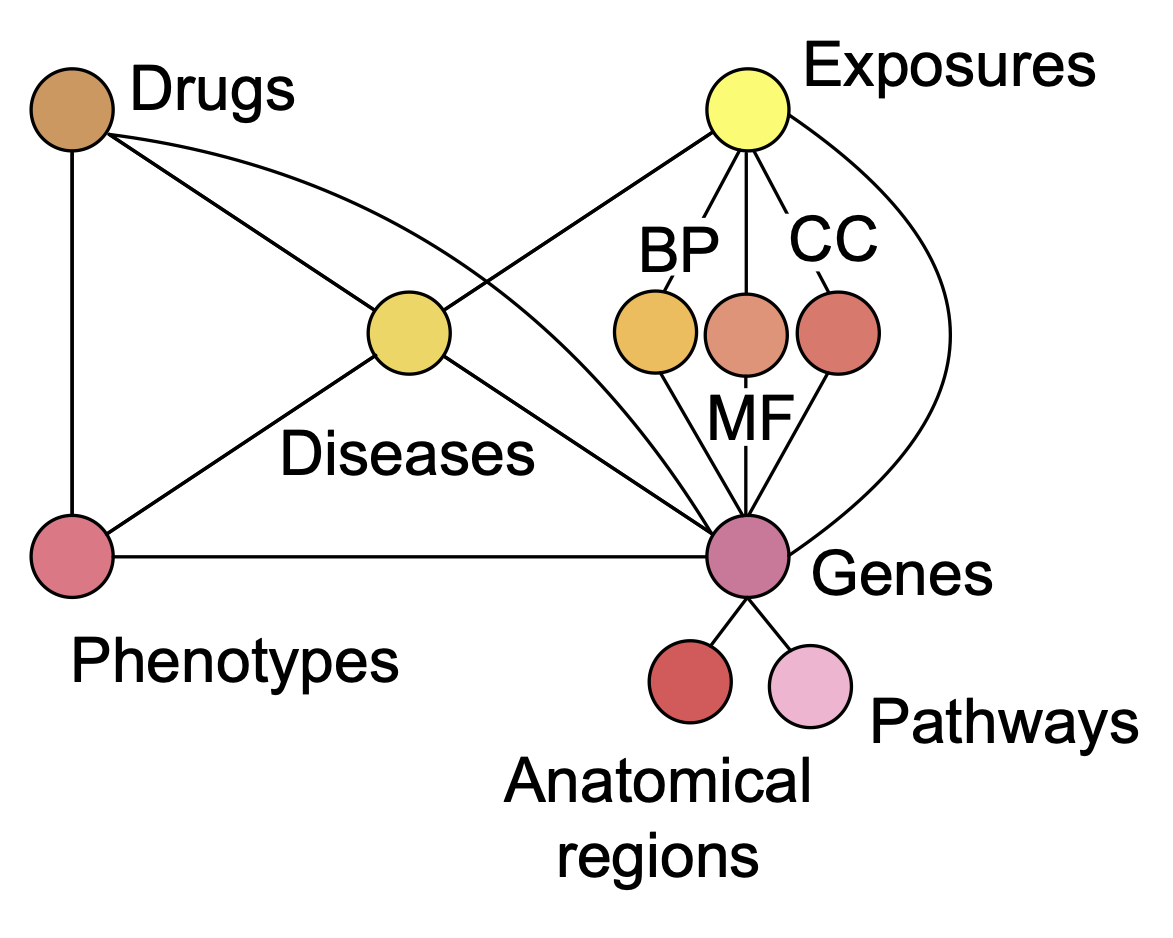
\includegraphics[width=0.6\textwidth]{figs/edge_types_hypergraph.png}
    \caption{Hypergraph of the edge types in PrimeKG}
    \label{fig:primekg_edge_types_hypergraph}
\end{figure}
To better understand the distribution of the edge types in PrimeKG, Figure~\ref{fig:primekg_edge_types_hypergraph_perc} illustrates the number of edges for each edge type by weighing the connections in the hypergraph according to their percentage in PrimeKG. Also, the directed hypergraph in Figure~\ref{fig:primekg_edge_types_hypergraph_perc_on_type} shows for each edge type the percentage of connections to the other edge types.
\begin{figure}
    \centering
    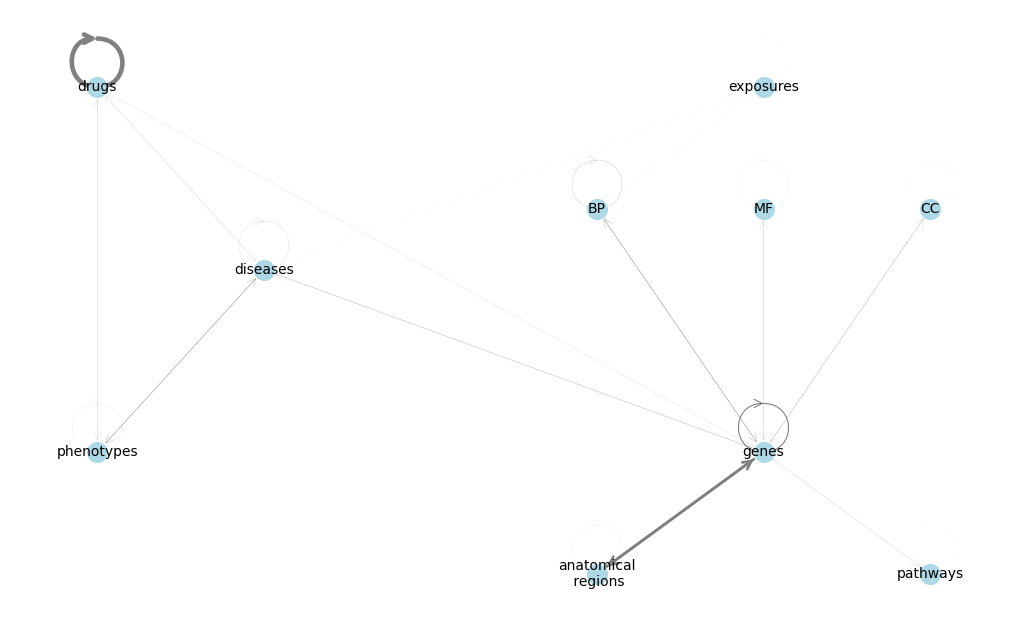
\includegraphics[width=0.6\textwidth]{figs/primekg_edge_types_perc.png}
    \caption{Hypergraph of the edge types in PrimeKG, with connections weighed according to their percentage in the graph}
    \label{fig:primekg_edge_types_hypergraph_perc}
\end{figure}
\begin{figure}
    \centering
    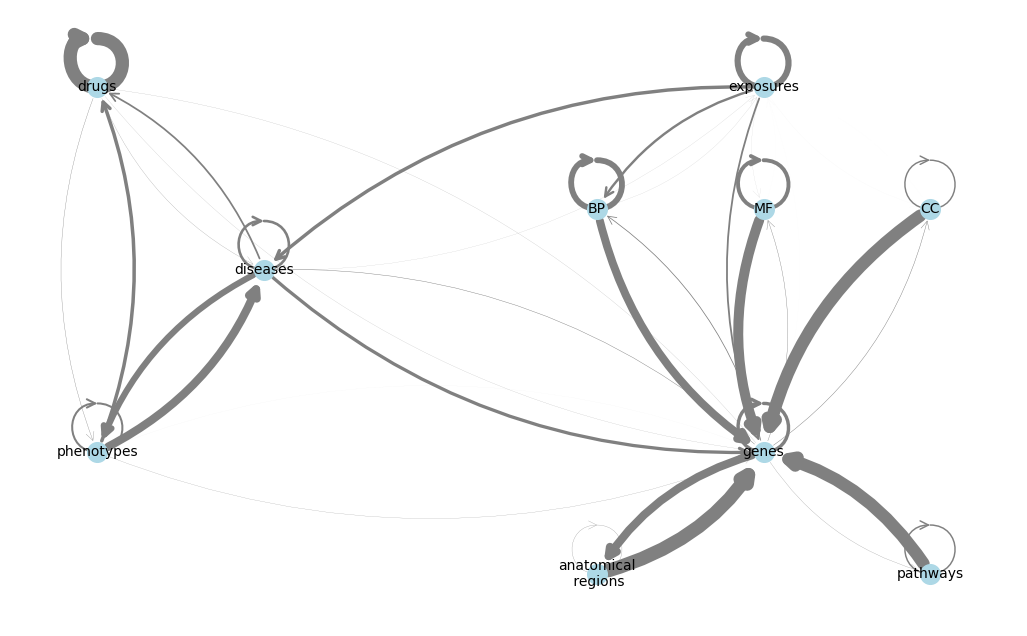
\includegraphics[width=0.6\textwidth]{figs/primekg_edge_types_perc_on_type.png}
    \caption{Hypergraph of the edge types in PrimeKG, with connections weighed according to their percentage in the graph}
    \label{fig:primekg_edge_types_hypergraph_perc_on_type}
\end{figure}

% \begin{table}
    \centering
    \begin{tabular}{rl}
        \toprule
        \textbf{Edge type} & \textbf{Number of edges}\\
        \midrule
        anatomy protein present & 3.036.406 \\
        drug drug & 2.672.628 \\
        protein protein & 642.150 \\
        disease phenotype positive & 300.634 \\
        bioprocess protein & 289.610 \\
        cellcomp protein & 166.804 \\
        disease protein & 160.822 \\
        molfunc protein & 139.060 \\
        drug effect & 129.568 \\
        bioprocess bioprocess & 105.772 \\
        pathway protein & 85.292 \\
        disease disease & 64.388 \\
        contraindication & 61.350 \\
        drug protein & 51.306 \\
        anatomy protein absent & 39.774 \\
        phenotype phenotype & 37.472 \\
        anatomy anatomy & 28.064 \\
        molfunc molfunc & 27.148 \\
        indication & 18.776 \\
        cellcomp cellcomp & 9.690 \\
        phenotype protein & 6.660 \\
        off-label use & 5.136 \\
        pathway pathway & 5.070 \\
        exposure disease & 4.608 \\
        exposure exposure & 4.140 \\
        exposure bioprocess & 3.250 \\
        exposure protein & 2.424 \\
        disease phenotype negative & 2.386 \\
        exposure molfunc & 90 \\
        exposure cellcomp & 20 \\
        \bottomrule
    \end{tabular}
    \caption{Number of edges for each edge type in Prime KG}\label{tab:primekg_edge_types}
\end{table}
% ~\ref{tab:primekg_edge_types}.



\section{Patient data}\label{data_sources:patient_data}